%%%%%%%%%%%%%%%%%%%%%%%%%%%%%%%%%%%%%%%%%%%%%%%%%%%%%%%%%%%%%%%%%%%%%%%%%%%%%%%%
%2345678901234567890123456789012345678901234567890123456789012345678901234567890
%        1         2         3         4         5         6         7         8

\documentclass[letterpaper, 10 pt, conference]{ieeeconf}  
\usepackage[utf8]{inputenc}

%\documentclass[a4paper, 10pt, conference]{ieeeconf}      % Use this line for a4
                                                          % paper

\IEEEoverridecommandlockouts                              
\overrideIEEEmargins

\usepackage{graphics}
\usepackage{epsfig} 
\usepackage{mathptmx} 
\usepackage{times} 
\usepackage{amsmath}
\usepackage{amssymb}
\usepackage{fancyhdr}
\usepackage{hyperref}
\pagestyle{fancy}
\fancyhf{}

\title{\LARGE \bf
Comunicación Serial
}

\author{Socasi Bryan$^{1}$, Viera Khaterine$^{2}$, Yánez Danilo$^{3}$% <-this % stops a space
}




\begin{document}

\maketitle
\thispagestyle{empty}
\pagestyle{empty}
\fancyfoot[]{Universidad de las Fuerzas Armadas "ESPE"}
%%%%%%%%%%%%%%%%%%%%%%%%%%%%%%%%%%%%%%%%%%%%%%%%%%%%%%%%%%%%%%%%%%%%%%%%%%%%%%%%
\begin{abstract}

This project consists of applying a serial communication between computers to control sensors and actuators that are connected to Arduino cards. The communication must be bidirectional and crossed, this means that the software of the sensors must be able to receive the data to activate the sensors and the softaware for the sensors must be able to receive the data to activate the sensors.

\end{abstract}


%%%%%%%%%%%%%%%%%%%%%%%%%%%%%%%%%%%%%%%%%%%%%%%%%%%%%%%%%%%%%%%%%%%%%%%%%%%%%%%%
\section{INTRODUCCIÓN}

La evolución de la tecnología en las últimas décadas ha permitido generar nuevos protocolos y dispositivos para la transmisión de datos entre una computadora y un periférico,en sus inicios alrededor de los años 60 esta transmisión de información se daba a través de puertos seriales enviando datos bit a bit con tiempo de espera prolongado, después en1998 fue reemplazada por puertos USB’s que tenían mejores características y mayor eficiencia. Actualmente los individuos no tienen pleno conocimiento sobre los fundamentos o la estructura base que permitió que la comunicación pueda darse como se la conoce ahora,sin embargo, es muy importante entender los inicios en esta área especialmente para los estudiantes de ingeniería en electrónica, pues de esta manera se logrará entender la diversidad que ha existido a lo largo del tiempo y cómo funciona cada “cosa” que utilizamos.Relacionando los temas aprendidos en clase se desarrolla un trabajo de investigación que involucra la comunicación serial entre dos PC a través de una interfaz gráfica desarrollada con lenguaje de programación Java, controlada por un arduino.

\section{CONCEPTOS}

\subsection{Arduino UNO}

Arduino UNO es una placa electrónica basada en el microcontrolador ATmega 328. Cuenta con 14 pines digitales que pueden ser entradas o salidas de los cuales 6 pueden ser usados como salidas PWM, 6 entradas analógicas, un cristal oscilador de 16 MHz, una conexión USB,un conector de alimentación, una cabecera ICSP y un botón de reinicio.
\begin{center}
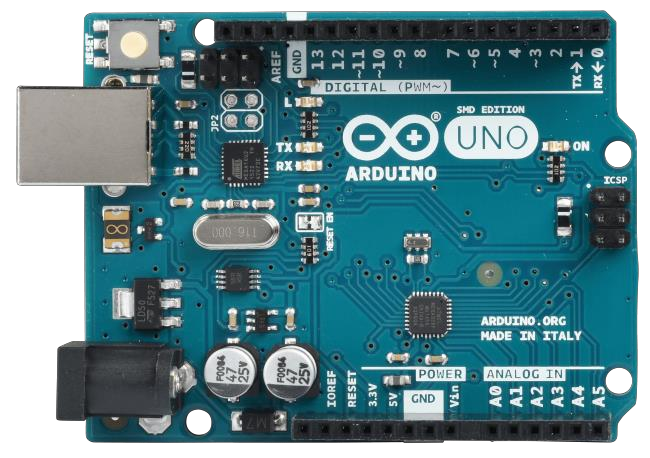
\includegraphics[scale=0.3]{Documento/Figuras/fig1.png}
\begin{scriptsize}\\ 
Fig 1. Arduino Uno
\end{scriptsize}
\end{center}

\subsection{Definición de pines}
\begin{center}
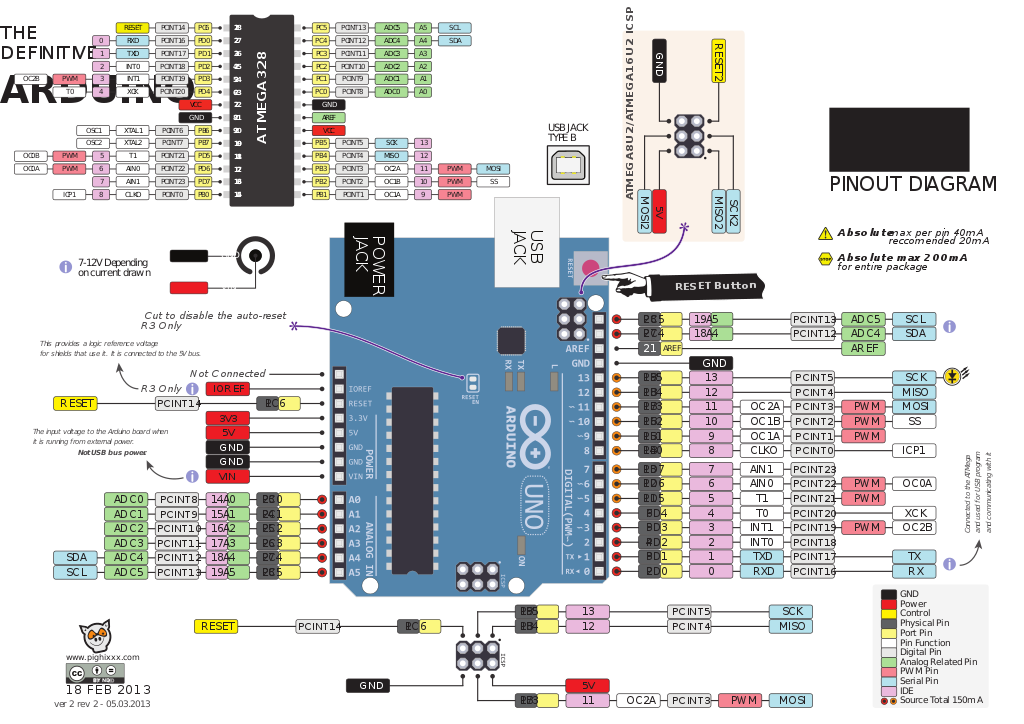
\includegraphics[scale=0.2]{Documento/Figuras/fig2.png}
\begin{scriptsize}\\ 
Fig 1. Definición de pines Arduino Uno
\end{scriptsize}
\end{center}

\subsection{Java}

Es un lenguaje de programación de propósito general, concurrente, orientado a objetos que fue diseñado específicamente para tener tan pocas dependencias de implementación como fuera posible. Su intención es permitir que los desarrolladores de aplicaciones escriban el programa una vez y lo ejecuten en cualquier dispositivo, lo que quiere decir que el código que es ejecutado en una plataforma no tiene que ser recompilado para correr en otra. Java es, a partir de 2012, uno de los lenguajes de programación más populares en uso, particularmente para aplicaciones de cliente-servidor de web.
\begin{center}

\includegraphics[scale=0.2]{Documento/Figuras/fig3.png}
\begin{scriptsize}\\ 
Fig 2. Lenguaje de Programación JAVA
\end{scriptsize}
\end{center}

\subsection{API Java Communications}

La API de Java Communications es una extensión de Java que facilita el desarrollo de aplicaciones de comunicaciones independientes de plataforma para tecnologías como Smart Cards, sistemas integrados y dispositivos de punto de venta, dispositivos de servicios financieros, fax, módems, terminales de pantalla y equipos robóticos.
La API de comunicaciones de Java también conocida como javax.comm permite a las aplicaciones el acceso al hardware RS-232 (puertos serie) y un acceso limitado a IEEE-1284 (puertos paralelos), modo SPP. (Itcea, 2017)

\subsubsection{Características}
 \begin{itemize}
     \item Enumeración de puertos (mapeo de puertos configurables por el administrador y el usuario)
     \item Configuración del puerto (velocidad en baudios, velocidad, bits de parada, paridad)
     \item Acceso a señales estándar DTR, CD, CTS, RTS y DSR EIA232
     \item Transferencia de datos a través de puertos RS-232
     \item Opciones de control de flujo de hardware y software.
     \item 	Control de umbral de buffer de recepción.
     \item Opción de evento asincrónico para la notificación de:
     \begin{itemize}
         \item Datos disponibles en un puerto RS232.
         \item Cambios de nivel de línea de hardware de puerto.
         \item Cambios en la propiedad de puerto de una solo JVM.
     \end{itemize}
 \end{itemize}

\subsection{Sensores}

Es un concepto genérico que hace referencia a diferentes tipos de sensores, esto se entiende tanto las unidades que emite una señal analógica, como las unidades que emite una señal binaria (encendido o apagado).

\begin{center}
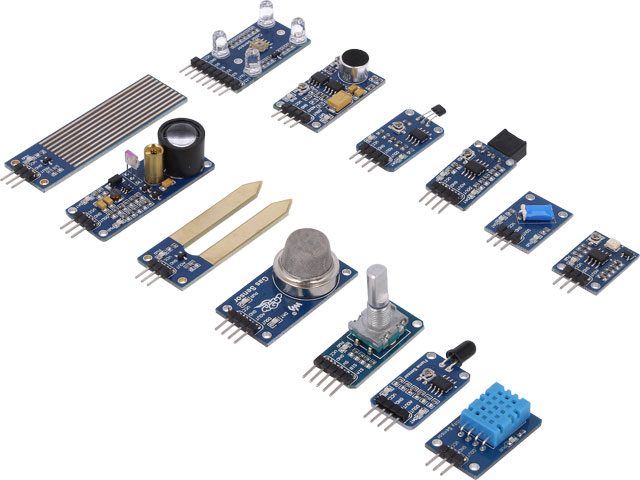
\includegraphics[scale=0.25]{Documento/Figuras/fig4.jpg}
\begin{scriptsize}\\ 
Fig 3. Sensores Electrónicos.
\end{scriptsize}
\end{center}

Convierte una magnitud física en una magnitud eléctrica, existe una gama de diferentes productos de sensores para diferentes magnitudes físicas.


\section{Diagramas}
\subsection{Diagrama de bloques}

 \begin{center}
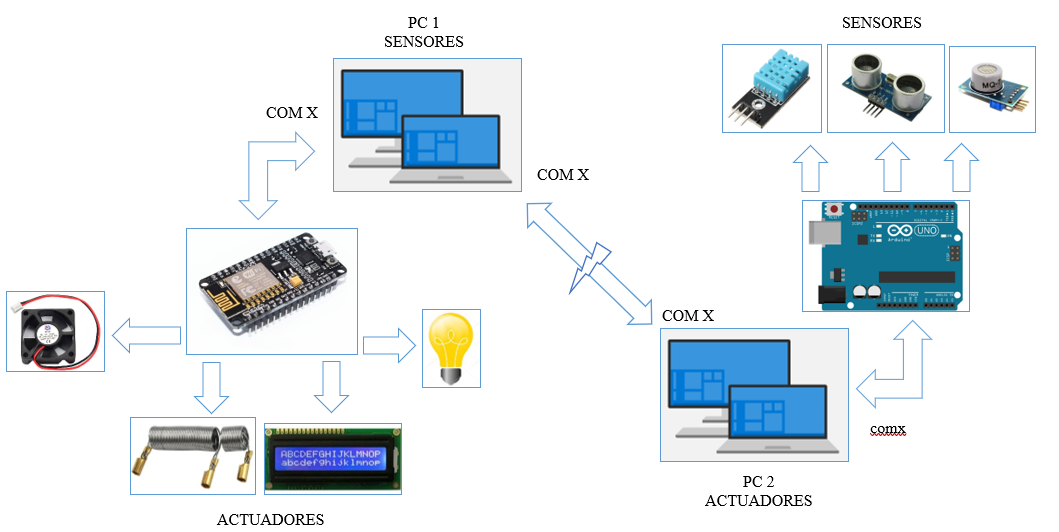
\includegraphics[scale=0.3]{Documento/Figuras/fig8.PNG}
\begin{scriptsize}\\ 
Fig 8. Diagrama de bloques de la Comunicación Serial
\end{scriptsize}
\end{center}


\section{ESTADO DEL ARTE}
\subsection{Java}
En (Cisco systems, 2016) se indica qué es Java y su programación orientada a objetos, elementos del lenguaje Java, operadores y estructuras de control del lenguaje Java, fundamentos de definición y uso de clases, sistema, cadenas, cadena de buffer, math y otras clases de envoltura, arrays, clases y herencia, cómo comprender y usar los paquetes, creación de interfaces gráficas de usuario con AWT, applets y gráficos, excepciones, archivos, flujos, entrada y salida, colecciones, hilos.

\subsection{Arduino}
En (Albatish, Mosa, & Abu , 2018) se encontró información sobre cómo enfrentar alguna dificultad al tratar con la plataforma Arduino mediante la descripción del diseño de un sistema de tutoría inteligente basado en escritorio. La idea principal de este sistema es una introducción sistemática al concepto de plataforma Arduino. El sistema muestra las placas de circuito de Arduino y un entorno de desarrollo de fuente abierta y una biblioteca para escribir código para controlar el tema de la placa de la plataforma Arduino.
Lo que nos indica en (Pan & Zhu, 2018) es que un sensor es "un dispositivo que detecta una variación en la energía de entrada para producir una variación en otra o la misma forma de energía". Por tanto, implementarlos con arduino, es una manera muy interesante de realizar este tipo de proyectos, de esta manera, en este artículo se describe aspectos importantes de su uso.\\

\subsection{Comunicación Serial}
En el artículo de (Padrón, Prieto, Herrera, & Velazquez, 2018) se indica una aplicación importante con la comunicación serial pues debido a la naturaleza inherente a las comunicaciones móviles, diversos factores influyen en la calidad de los servicios que se desarrollan para los dispositivos de enlace cuando son fabricados, en los cuales no se encuentran técnicas y procedimientos de seguridad implementados en comparación con dispositivos fijos o de escritorio actuales. En este trabajo se presenta la implementación del algoritmo criptográfico por bloques "Advanced Encryption Standard" (AES) de 128 bits, para una comunicación serial entre dos tarjetas Spartan 3E fabricadas por Xilinx. Este algoritmo público según la FIPS-197 es el estándar para muchas aplicaciones en Seguridad Informática tanto en Software como Hardware. Este método criptográfico sigue siendo un mecanismo para implementar los servicios de seguridad recomendados en la ISO 7498-2.

\section{EXPLICACIÓN DEL CÓDIGO}
\subsection{Comunicación Serial}
Usaremos el API Java Communications (COMM) que nos permitirá manejar el puerto serie, y así comunicarnos con el otro computador. 
También usaremos cables adaptadores USB a DB9 y el más importante, un cable DB9 cruzado para que el envió de bits se realice correctamente.
Para usar el api de comunicaciones de java necesitaremos de una librería que contiene las clases para manejar los puertos, estos archivos se deben incluir en la carpeta donde se encuentra el Java instalado, siguiendo las siguientes direcciones:
\begin{itemize}
    \item Comm.jar \textbackslash jdk\textbackslash jre\textbackslash lib\textbackslash ext
    \item Win32com.dll  \textbackslash jdk\textbackslash bin y en \textbackslash Windows\textbackslash system32
    \item Javax.comm.properties \textbackslash jdk\textbackslash jre\textbackslash lib
\end{itemize}
	
Para el código necesitaremos importar la librería mencionada anteriormente
\\
\begin{center}
    import javax.comm.*; 
\end{center}
\\
A continuación tenemos que declarar las clases necesarias para manejar los puertos con sus respectivas variables asignadas, hay que tener en cuenta que la comunicación que usaremos es FULL-DUPLEX, ya que enviaremos y recibiremos información entre ambos computadores.
\begin{center}
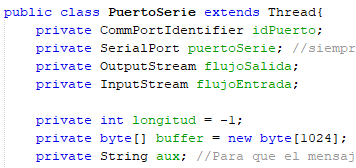
\includegraphics[scale=0.8]{Documento/Figuras/1.PNG}
\begin{scriptsize}
\\ 
\end{scriptsize}
\end{center}

\begin{center}
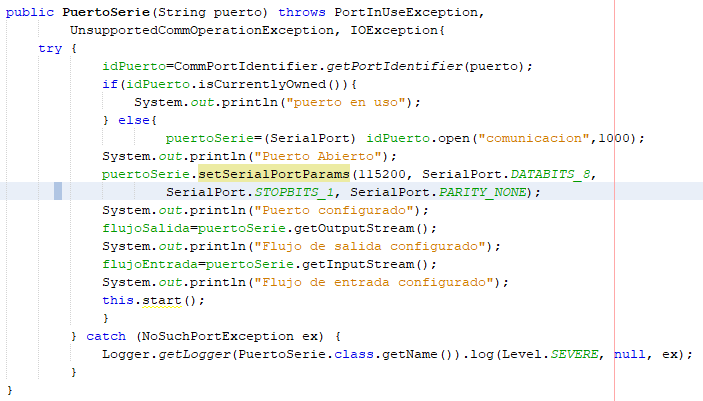
\includegraphics[scale=0.42]{Documento/Figuras/2.PNG}
\begin{scriptsize}
\\ 
\end{scriptsize}
\end{center}
Para la transmisión de información, declararemos un método con un argumento para transmitir el mensaje deseado, nos ayudaremos de un método .write() que posee la clase SerialPort.
\begin{center}
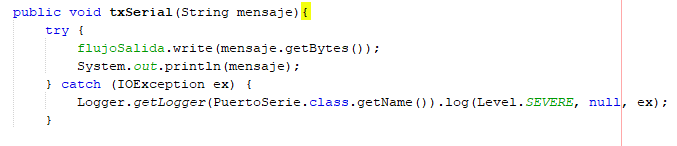
\includegraphics[scale=0.46]{Documento/Figuras/3.PNG}
\begin{scriptsize}
\\ 
\end{scriptsize}
\end{center}
Ahora para recibir datos usaremos un método run() de la clase derivada de Thread que nos permitirá crear un subproceso en el programa y con esto poner al puerto en constante “escucha”, por lo que necesitaremos crear un hilo hacia el constructor que contiene la información del puerto usado.
\begin{center}
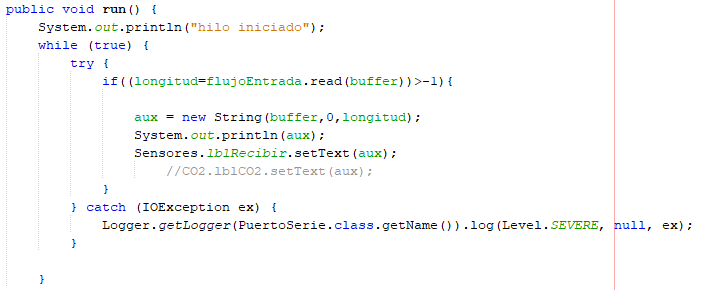
\includegraphics[scale=0.45]{Documento/Figuras/4.PNG}
\begin{scriptsize}
\\ 
\end{scriptsize}
\end{center}
Como usaremos varios sensores y actuares es necesario comunicarse con estos a través del puerto y luego cerrar dicha comunicación, ya que si esta quedara abierta, seria imposible comunicarse con varios sensores o actuadores a la vez, por lo que es necesario crear un método para cerrar los puertos usados.
\begin{center}
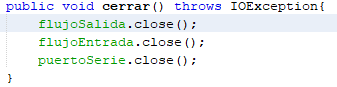
\includegraphics[scale=0.94]{Documento/Figuras/5.PNG}
\begin{scriptsize}
\\ 
\end{scriptsize}
\end{center}
Ahora necesitamos crear un Jframe para el control de esta clase, para este proyecto es necesario dos GUIs una que controlara los sensores y otra para controlar los actuadores.
Básicamente necesitamos colocar un ComboBox con el nombre de los puertos y un botón para activar la comunicación.
En el botón agregaremos un evento para que realice una acción al momento de ser presionado, esto nos permitirá escribir el código para activar la comunicación, para lo cual primero debemos crear un objeto de la clase que contiene los parámetros del Puerto serie y luego llamar los métodos necesarios para iniciar la comunicación, llevando la información obtenida del ComboBox y el mensaje deseado al momento de presionar el botón.
\begin{center}
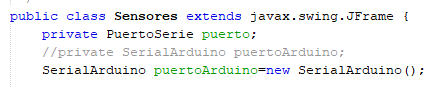
\includegraphics[scale=0.7]{Documento/Figuras/6.PNG}
\begin{scriptsize}
\\ 
\end{scriptsize}
\end{center}
\begin{center}
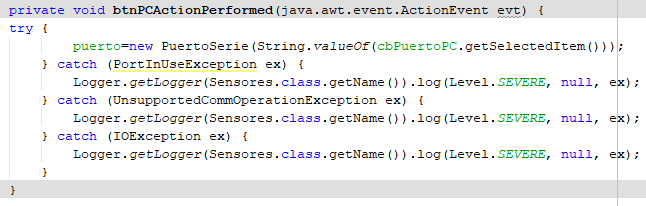
\includegraphics[scale=0.45]{Documento/Figuras/7.PNG}
\begin{scriptsize}
\\ 
\end{scriptsize}
\end{center}

\section{CÓDIGO ARDUINO}
\subsubsection{Actuadores}
\begin{center}
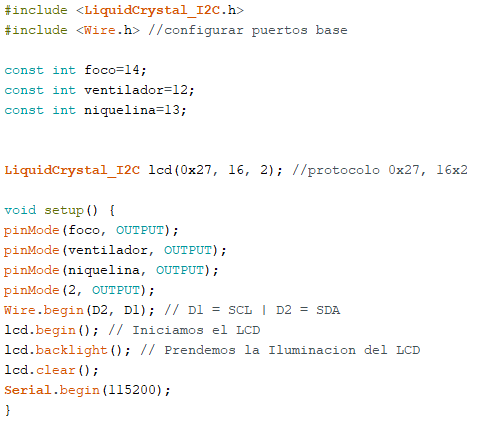
\includegraphics[scale=0.65]{Documento/Figuras/10.PNG}
\begin{scriptsize}
\\ 
\end{scriptsize}
\end{center}
\begin{center}
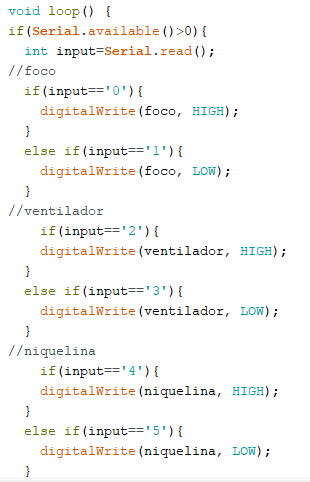
\includegraphics[scale=0.8]{Documento/Figuras/11.PNG}
\begin{scriptsize}
\\ 
\end{scriptsize}
\end{center}

\subsection{Sensores}
\begin{center}
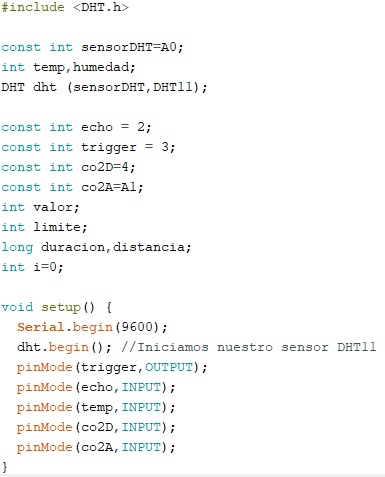
\includegraphics[scale=0.8]{Documento/Figuras/12.PNG}
\begin{scriptsize}
\\ 
\end{scriptsize}
\end{center}
\begin{center}
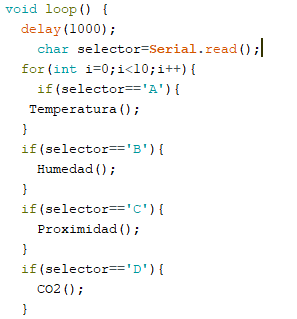
\includegraphics[scale=0.8]{Documento/Figuras/13.PNG}
\begin{scriptsize}
\\ 
\end{scriptsize}
\end{center}
\begin{center}
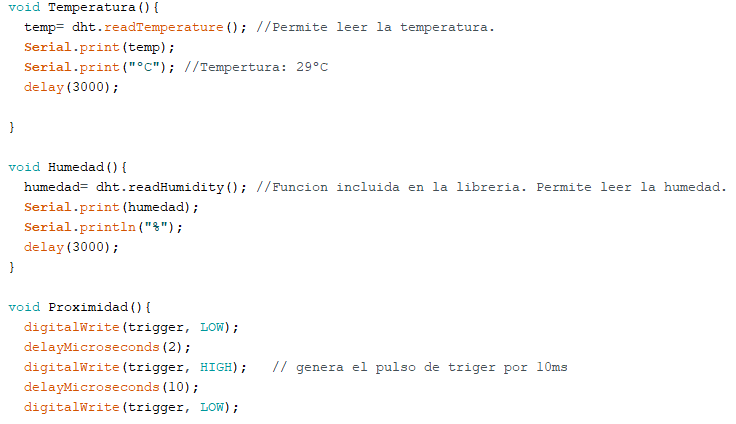
\includegraphics[scale=0.45]{Documento/Figuras/14.PNG}
\begin{scriptsize}
\\ 
\end{scriptsize}
\end{center}

\section{CONCLUSIONES}
  \begin{itemize}

   \item La comunicación de puerto serial ha tenido una breve evolución en las últimas décadas, a través del estado del arte se comprobó su aplicación y funcionamiento con la transmisión de datos, en la creación del sistema de comunicación serial presentado en este informe, se procedió a la conexión entre dos computadoras con el Arduino y el uso del ESP8266, enviando datos para realizar la comunicación serial tanto para los sensores y los actuadores, por medio de una consola de java y Arduino.
     \item El Arduino se puede utilizar para diferentes ámbitos como desarrollar elementos autónomos, conectándose a dispositivos e interactuar tanto con el hardware como con el software; es una plataforma electrónica que en este trabajo nos permitió la interacción con una interfaz gráfica desarrollada con lenguaje de programación Java, con la finalidad de poder tener una interacción más fácil del Arduino con el computador.
     \item Se logro cumplir con cada uno de los objetivos, y entender el desarrollo de todos los programas, implementados en dos computadoras, con el debido funcionamiento de los Sensores y Actuadores.
  \end{itemize}

\addtolength{\textheight}{-12cm}   

\section{RECOMENDACIONES}
\begin{itemize}
    \item Se debe considerar que los pines en los que se conecta cada uno de los sensores y actuadores, que están configurados para funcionar en un orden específico, para obtener los datos requeríos en el Producto de unidad.
    \item Se debe tener en consideración que los paquetes utilizados en Java, no son propios de ahí, pero se debe descargar las librerias, y el funcionamiento de código nos permita trabajar de manera eficaz en los programas implementados..
    \item Conectar correctamente nuestros elementos, tanto a la tarjeta de Desarrollo del ESP8266 y la tarjeta de desarrollo Arduino UNO, debido a que, aunque realicemos correctamente la programación y la configuración con el servidor, los Actuadores y sensores se encuentran en los pines incorrectos o con la polarización indebida estos no podrán funcionar como esperamos.
\end{itemize}

\begin{thebibliography}{99}

\bibitem{1}A., P. (17 de 10 de 2012). twenergy. Recuperado el 04 de 28 de 2018, de https://twenergy.com/a/como-se-genera-la-electricidad-666

\bibitem{2}Albatish, I., Mosa, M., & Abu , S. (01 de 2018). ResearchGate. Obtenido de 323322871_ARDUINO_Tutor_An_Intelligent_Tutoring_System

\bibitem{3}BBVA Open4U. (15 de 08 de 2015). BBVA. Obtenido de https://bbvaopen4u.com/es/actualidad/el-internet-de-las-cosas-de-codigo-abierto-plataformas-y-aplicaciones-para

\bibitem{4}Carlos, C. (12 de 06 de 2015). Galia,FC. Obtenido de http://galia.fc.uaslp.mx/

\bibitem{5}Cisco systems. (03 de 2016). ResearchGate. Obtenido de https://www.researchgate.net/publication/

\bibitem{6}Crespo, E. (25 de 09 de 2016). Aprendiendo Arduino. Obtenido de https://aprendiendoarduino.wordpress.com/2016/09/25/que-es-arduino/

\bibitem{7} Facultad Tecnológica. (02 de 10 de 2014). Universidad Distrital Francisco José de Caldas. Recuperado el 28 de 04 de 2018, de http://gemini.udistrital.edu.co/comunidad/grupos/gispud/Circuitos-II/Capitulo-3/3.2.1.html

\bibitem{8}García, J. A. (s.f.). AF. Obtenido de AF: http://www.asifunciona.com/fisica/af_diodos/af_diodos_6.htm

\bibitem{9}N.O.Sadiku, C. K. (2013). En Fundamentos de Circuitos Eléctricos (pág. 866). México: Mc Graw Hill Education
\end{thebibliography}


\end{document}
